\documentclass[10pt]{beamer}
\usetheme{jambro}

\title[]{Pensamento Econômico Contemporâneo - A escola monetarista ortodoxa}
\author[]{Paulo Victor da Fonseca}
\date{}

\hypersetup{
    colorlinks = true,
    urlcolor = teal,
    linkcolor = teal    
}
\usepackage[portuguese]{babel}
\usepackage{subfig}
\usepackage{emoji}

\begin{document}

\begin{frame}[plain]
    \titlepage{
        \begin{center}
            \begin{minipage}{0.8\textwidth}
                \centering
            \end{minipage}
        \end{center}}
\end{frame}

\begin{frame}{Sumário}
    \tableofcontents
\end{frame}

\section{TQM e renda nominal: evidência empírica}
\begin{frame}{TQM e variações na renda nominal: evidência empírica}
    \begin{itemize}
        \item $\exists$ \textcolor{purple}{de relação funcional estável entre demanda por encaixes reais e um nº limitado de variáveis que a determinam}: abordagem moderna da TQM
        \bigskip
        \item Demanda por moeda estável $\Rightarrow$ velocidade também estável e variará de maneira previsível no caso em que qualquer argumento da função de demanda por moeda for alterada
    \end{itemize}
\end{frame}

\begin{frame}{TQM e variações na renda nominal: evidência empírica}
    \begin{itemize}
        \item Friedman postulou a TQM como
    \end{itemize}
    \NB{
        A generaliza\c{c}\~{a}o emp\'{i}rica de que varia\c{c}\~{o}es nos encaixes reais desejados (na demanda por moeda) tendem a ocorrer de maneira lenta e gradual ou ser o resultado de eventos desencadeados por mudan\c{c}as na oferta ao passo que, em contraste, varia\c{c}\~{o}es significativas na oferta de encaixes nominais podem e frequentemente ocorrem de maneira independente de qualquer varia\c{c}\~{a}o na demanda. \textcolor{purple}{A conclus\~{a}o \'{e} que varia\c{c}\~{o}es significativas nos pre\c{c}os ou na renda nominal s\~{a}o, quase que invariavelmente, resultados de mudan\c{c}as na oferta nominal de moeda}    
    \begin{flushright}
    (Friedman, 1968)
    \end{flushright}}
\end{frame}

\begin{frame}{TQM e variações na renda nominal: evidência empírica}
    \begin{itemize}
        \item Objetivo: discutir evidências empíricas que suportam abordagem da TQM, começando com a função de demanda por moeda
        \bigskip
        \item Dois pontos merecem ser destacados:
        \bigskip
        \item[(1)] Friedman (1959) afirma que em seus trabalhos empíricos encontrou que a taxa de juros era insignificante para a demanda por moeda, no entanto, praticamente todos os estudos subsequentes mostraram que a taxa de juros era uma variável importante na função de demanda por moeda
        \bigskip
        \item Tobin ``convenceu grande parte da profissão de que a demanda por moeda tem uma sensibilidade econômica- e estatisticamente significativa com relação à taxa de juros'' (LM não é perfeitamente inelástica)
    \end{itemize}
\end{frame}

\begin{frame}{TQM e variações na renda nominal: evidência empírica}
    \begin{itemize}
        \item Argumento importante para a prescrição de políticas fiscais discricionárias de estabilização advogadas por Tobin
        \bigskip
        \item Anos 1950s e 1960s: pouca evidência de que a elasticidade-juro da demanda por moeda aumentava à medida que a taxa de juros fosse reduzida, como requerido pela armadilha da liquidez
        \bigskip
        \item Portanto, podemos desconsiderar os dois casos extremos de LM vertical e horizontal
        \bigskip
        \item No entanto, IS-LM estático ainda pode ser usado para ilustrar a abordagem da TQM no caso em que a taxa real de juros e a renda real são determinados por forças reais, e não monetárias, e a economia tende automaticamente ao equilíbrio de pleno emprego
    \end{itemize}
\end{frame}

\begin{frame}{TQM e variações na renda nominal: evidência empírica}
    \begin{itemize}
        \item[(2)] Estabilidade da função de demanda por moeda sustentada empiricamente até início dos 1980s. Desde então, evidências de instabilidade aparente (EUA e outras economias)
    \end{itemize}
    \begin{figure}
        \centering
        \href{https://fred.stlouisfed.org/graph/?g=PNOQ}{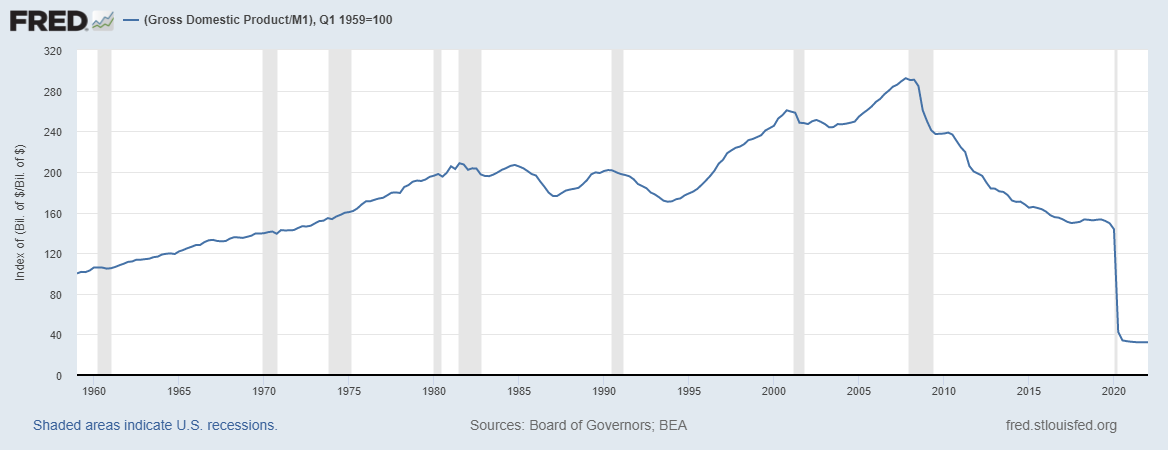
\includegraphics[width=0.9\textwidth]{./figures/aula10_fig1.png}}
        \caption{Velocidade nos EUA ($M1$). Fonte: \href{https://fred.stlouisfed.org/graph/?g=PNOQ}{St. Louis Fed.}}
        \label{fig1}
    \end{figure}
\end{frame}

\begin{frame}{TQM e variações na renda nominal: evidência empírica}
    \begin{itemize}
        \item Fig. \ref{fig1}: pré-1980s (ápice do monetarismo) com tendência previsível de crescimento na velocidade do agregado monetário restrito, $M1$
        \bigskip
        \item Pós-1980s parece haver uma quebra nesta tendência estável - velocidade passa a apresentar grandes oscilações
        \bigskip
        \item Basicamente isto reflete uma relação de demanda por moeda relativamente estável pré-1980 e uma relação instável desde então
    \end{itemize}
\end{frame}

\begin{frame}{TQM e variações na renda nominal: evidência empírica}
    \begin{itemize}
        \item Anos 1990s: quebra na estabilidade da velocidade percebida também para agregados monetários mais amplos como $M2$ e $M3$ - Figuras \ref{fig2} e \ref{fig3}
    \end{itemize}
    \begin{figure}
        \centering
        \href{https://fred.stlouisfed.org/graph/?g=PNQI}{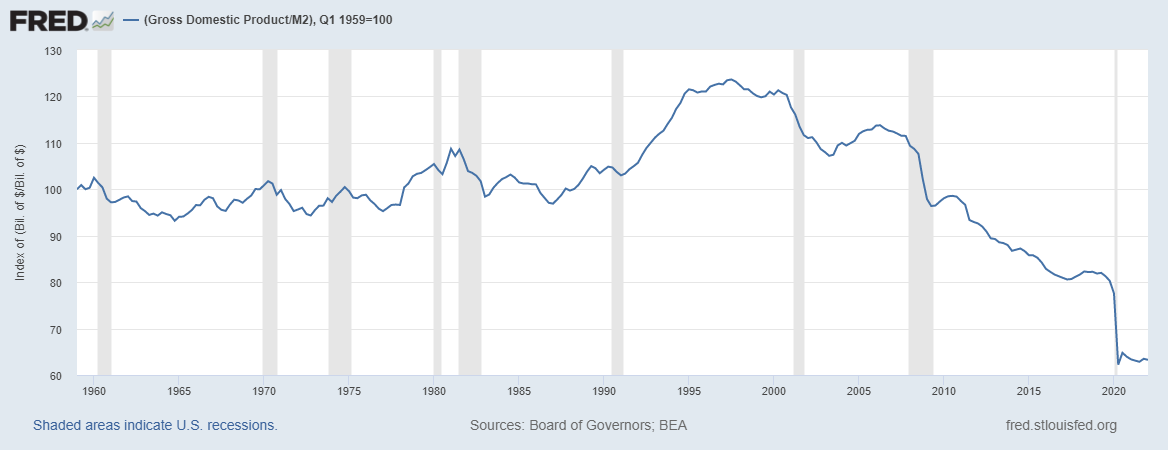
\includegraphics[width=\textwidth]{./figures/aula10_fig2.png}}
        \caption{Velocidade nos EUA ($M2$). Fonte: \href{https://fred.stlouisfed.org/graph/?g=PNQI}{St. Louis Fed.}}
        \label{fig2}
    \end{figure}
\end{frame}

\begin{frame}{TQM e variações na renda nominal: evidência empírica}
    \begin{figure}
        \centering
        \href{https://fred.stlouisfed.org/graph/?g=PNRb}{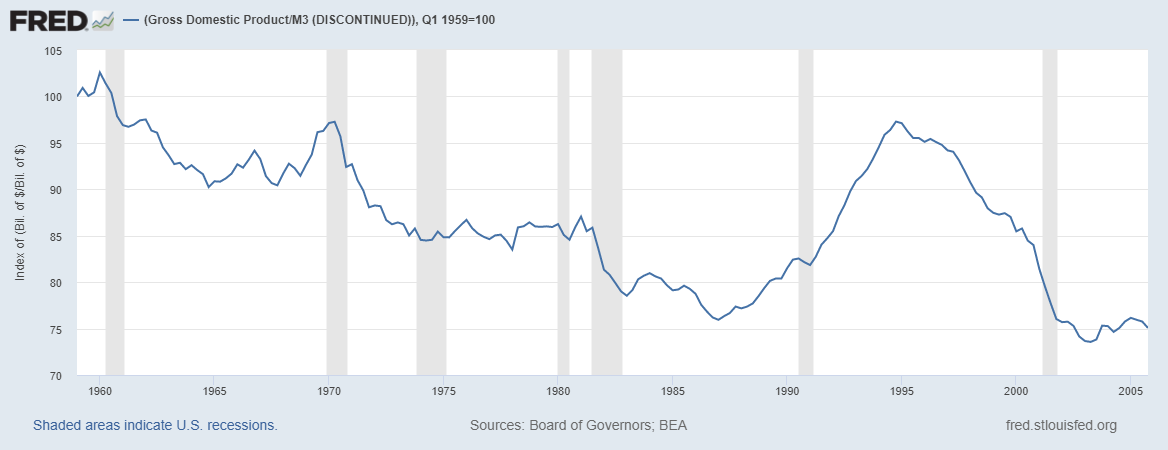
\includegraphics[width=0.9\textwidth]{./figures/aula10_fig3.png}}
        \caption{Velocidade nos EUA ($M3$). Fonte: \href{https://fred.stlouisfed.org/graph/?g=PNRb}{St. Louis Fed.}}
        \label{fig3}
    \end{figure}
    \begin{itemize}
        \item Explicações para aparente instabilidade: e.g., mudanças institucionais no sistema financeiro introduzidas nos anos 1970s e 1980s
    \end{itemize}
\end{frame}

\begin{frame}{TQM e variações na renda nominal: evidência empírica}
    \begin{itemize}
        \item Friedman (1958) tenta reestabelecer papel importante e independente para a moeda via estudos de séries temporais comparando as taxas de crescimento da moeda com os pontos de inflexão no nível de atividade econômica (EUA)
        \bigskip
        \item Em uma média de 18 ciclos analisados (períodos de paz pós-1870), picos (vales) na taxa de variação da oferta de moeda precederam picos (vales) no nível de atividade econômica por uma média de 16 (12) meses
        \bigskip
        \item Portanto, concluiu que este resultado fornecia uma forte evidência empírica de um canal de influência da moeda para o nível de atividade
    \end{itemize}
\end{frame}

\begin{frame}{TQM e variações na renda nominal: evidência empírica}
    \begin{itemize}
        \item Críticas metodológicas e estatísticas por Culbertson (1960, 1961) e Kareken e Solow (1963)
        \bigskip
        \begin{enumerate}
            \item Questionamento se a evidência temporal justificava a inferência de uma relação causal da moeda sobre o nível de atividade econômica
            \bigskip
            \item Objeções estatísticas: Friedman não comparou variáveis comparáveis
        \end{enumerate}
        \bigskip
        \item Kareken e Solow refazem os experimentos de Friedman utilizando taxas de variação para quantidade de moeda e nível de atividade econômica: não encontraram nenhuma evidência de liderança uniforme de variações monetárias sobre variações no nível de atividade econômica
    \end{itemize}
\end{frame}

\begin{frame}{TQM e variações na renda nominal: evidência empírica}
    \begin{itemize}
        \item Questão de causalidade da moeda sobre renda abordada por Tobin (1970), questiona a confiabilidade do protocolo temporal (leads e lags) das evidências empíricas de monetaristas
        \bigskip
        \item Com modelo `ultra Keynesiano', Tobin demonstrou como a evidência de protocolo temporal poderia ser interpretada em suporte às posições Keynesianas de ciclos e instabilidade
        \bigskip
        \item Friedman e falácia \emph{post hoc ergo propter hoc} (depois disso, logo, causado por isso)
        \bigskip
        \item Falácia da correlação coincidente: dois eventos que ocorram em sequência cronológica estão necessariamente interligados por uma relação de causa e efeito
    \end{itemize}
\end{frame}

\begin{frame}{TQM e variações na renda nominal: evidência empírica}
    \begin{itemize}
        \item Tobin ainda critica Friedman por não ter fundamento teórico explícito que ligasse a relação de causa e efeito que baseava proposições monetaristas
        \bigskip
        \item Para Tobin, trabalho de Friedman era ``mensuração sem teoria'' e, portanto, monetarismo permanecia, em grande parte, uma ``caixa preta''
        \bigskip
        \item Este problema de causalidade na macroeconomia levou, e ainda leva, a discussões e controvérsias sem fim na macro empírica
        \bigskip
        \item Discussão central na macro empírica: em 2011 Nobel de economia outorgado a Tom Sargent e Chris Sims por ``suas pesquisas empíricas sobre a causa e efeito na macroeconomia''
    \end{itemize}
\end{frame}

\begin{frame}{TQM e variações na renda nominal: evidência empírica}
    \begin{figure}
        \centering
        
\includegraphics[width=0.5\textwidth]{./figures/aula10_fig4.PNG}
        \caption{Tom Sargent e Chris Sims. Fonte: \href{https://www.nobelprize.org/prizes/economic-sciences/2011/summary/}{The Nobel Foundation.}}
        \label{fig4}
    \end{figure}
\end{frame}

\begin{frame}{TQM e variações na renda nominal: evidência empírica}
    \begin{itemize}
        \item Friedman e Schwartz (1963): evidências + persuasivas para argumento de que $\Delta$ no estoque de moeda tinha papel independente fundamental nas flutuações cíclicas de atividade
        \bigskip
        \item `\emph{Monetary history of the United States, 1867-1960}': enquanto o estoque de moeda tende a aumentar tanto em períodos de contração quanto de expansão no ciclo, a \hlight{taxa de crescimento da oferta de moeda} é menor em períodos de retração quando comparado com os de expansão da atividade
    \end{itemize}
\end{frame}

\begin{frame}{TQM e variações na renda nominal: evidência empírica}
    \begin{itemize}
        \item No período analisado, os únicos apresentaram queda absoluta do estoque de moeda foram os de maior contração econômica: 1873-9, 1893-4, 1907-8, 1920-1, 1929-33 e 1937-8
        \bigskip
        \item Além disso, Friedman e Schwartz argumentam que os fatores que causavam as contrações monetárias eram independentes de variações prévias ou contemporâneas na renda nominal e nos preços
        \bigskip
        \item Dito de outra forma, variações monetárias eram vistas como a causa, ao invés de consequência, das principais recessões econômicas
    \end{itemize}
\end{frame}

\begin{frame}{TQM e variações na renda nominal: evidência empírica}
    \begin{itemize}
        \item \textcolor{purple}{Grande Depressão:} um leve declínio inicial no estoque de moeda de 1929 a 1930 transformou-se em um forte declínio devido a uma onda de falências bancárias iniciada no final de 1930
        \bigskip
        \item Estas quebras nos bancos produziram um aumento tanto na razão moeda-depósitos devido à descrença do público na capacidade dos bancos em resgatar seus depósitos
        \bigskip
        \item Quanto um aumento na razão reserva-depósitos dado a descrença dos bancos na disposição do público em manter seus depósitos nas instituições
    \end{itemize}
\end{frame}

\begin{frame}{TQM e variações na renda nominal: evidência empírica}
    \begin{itemize}
        \item Para Friedman e Schwartz, a queda no estoque de moeda foi intensificado pela ação restritiva do Fed de aumentar a taxa de desconto em 1931 que, por sua vez, levou a mais quebras bancárias
        \bigskip
        \item A depressão econômica só tornou-se grande como resultado da incapacidade do Fed em impedir uma queda significativa no estoque de moeda - entre Outubro de 1929 e Junho de 1933 o estoque de moeda caiu 1/3 - Figura \ref{fig5}
    \end{itemize}
\end{frame}

\begin{frame}{TQM e variações na renda nominal: evidência empírica}
    \begin{figure}
        \centering
        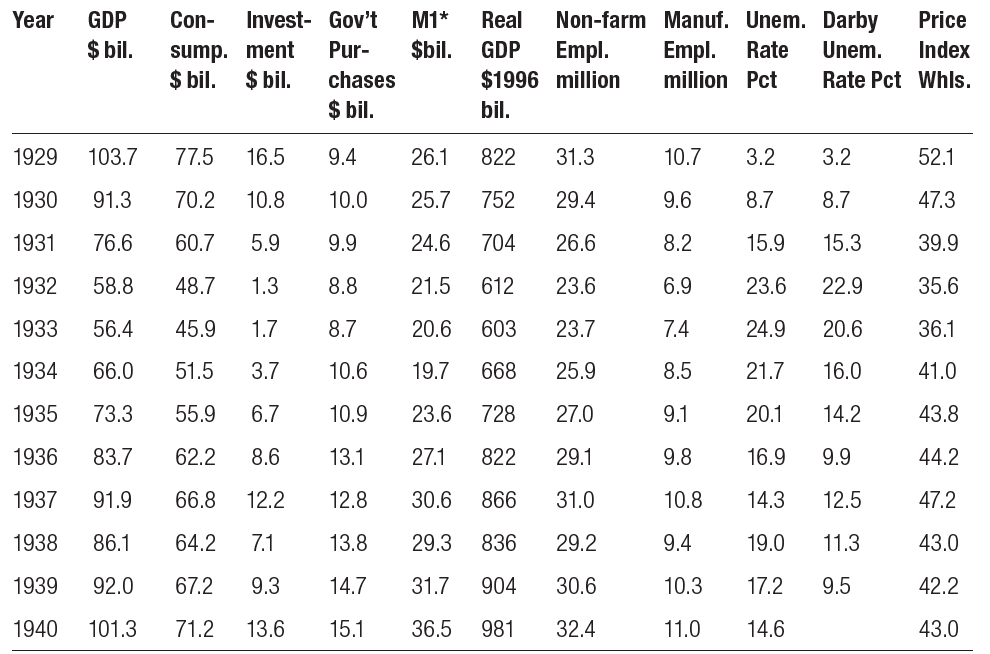
\includegraphics[width=0.7\textwidth]{./figures/aula10_fig5.PNG}
        \caption{Variáveis macroeconômicas, EUA (1929-1940). Fonte: McDonald (2022).}
        \label{fig5}
    \end{figure}
\end{frame}

\begin{frame}{TQM e variações na renda nominal: evidência empírica}
    \begin{itemize}
        \item Caso tivesse adotado políticas alternativas o Fed poderia ter evitado o colapso bancário e a resultante queda no estoque de moeda e contração econômica severa
        \bigskip
        \item Friedman e Schwartz justificam sua visão, subsequentemente, de que $\Delta$ no estoque de moeda tem papel independente fundamental nas flutuações cíclicas com a evidência de que movimentos cíclicos na moeda apresentavam, em grande parte, a mesma relação (em termos temporais e de amplitude) que os movimentos cíclicos de atividade, mesmo sob diferentes arranjos monetários adotados nos EUA ao longo de 1867-1960
    \end{itemize}
\end{frame}

\begin{frame}{TQM e variações na renda nominal: evidência empírica}
    \begin{itemize}
        \item Friedman e Meiselman (1963) tentam estimar quanto da $\Delta$ no consumo (proxy para a renda) pode ser explicada por variações:
        \bigskip
        \begin{enumerate}
            \item Na oferta de moeda - em linha com a TQM
            \bigskip
            \item No gasto autônomo (investimento) - em linha com a análise Keynesiana
        \end{enumerate}
        \bigskip
        \item Com duas equações para o teste econométrico (uma usando a moeda e a outra usando o gasto autônomo como variável independente) com dados EUA 1897-1957, encontraram que, com exceção de um subperíodo dominado pela Grande Depressão, a equação da moeda apresentava um resultado melhor
        \bigskip
        \item Resultados questionados por De Prano e Mayer (1965) e Ando e Modigliani (1965), que mostraram que uma alteração na definição de gasto autônomo melhorava a performance econométrica da equação de gasto autônomo
    \end{itemize}
\end{frame}

\begin{frame}{TQM e variações na renda nominal: evidência empírica}
    \begin{itemize}
        \item Cabe ressaltar que testes econométricos de Friedman e Meiselman foram mal formulados para discriminar entre a TQM e a visão Keynesiana, de forma que falharam em estabelecer se eram variações na oferta de moeda ou no gasto autônomo que causavam variações na renda
        \bigskip
        \item Isso pode ser ilustrado utilizando o modelo IS-LM para uma economia fechada
        \bigskip
        \item Em geral, no modelo IS-LM Hicksiano, os multiplicadores fiscais e monetários dependem da função consumo e da função de preferência pela liquidez
        \bigskip
        \item Resultados igualmente satisfatórios podem ser obtidos usando as duas equações quando a determinação da renda é puramente clássica ou puramente Keynesiana
    \end{itemize}
\end{frame}

\begin{frame}{TQM e variações na renda nominal: evidência empírica}
    \begin{figure}
        \centering
        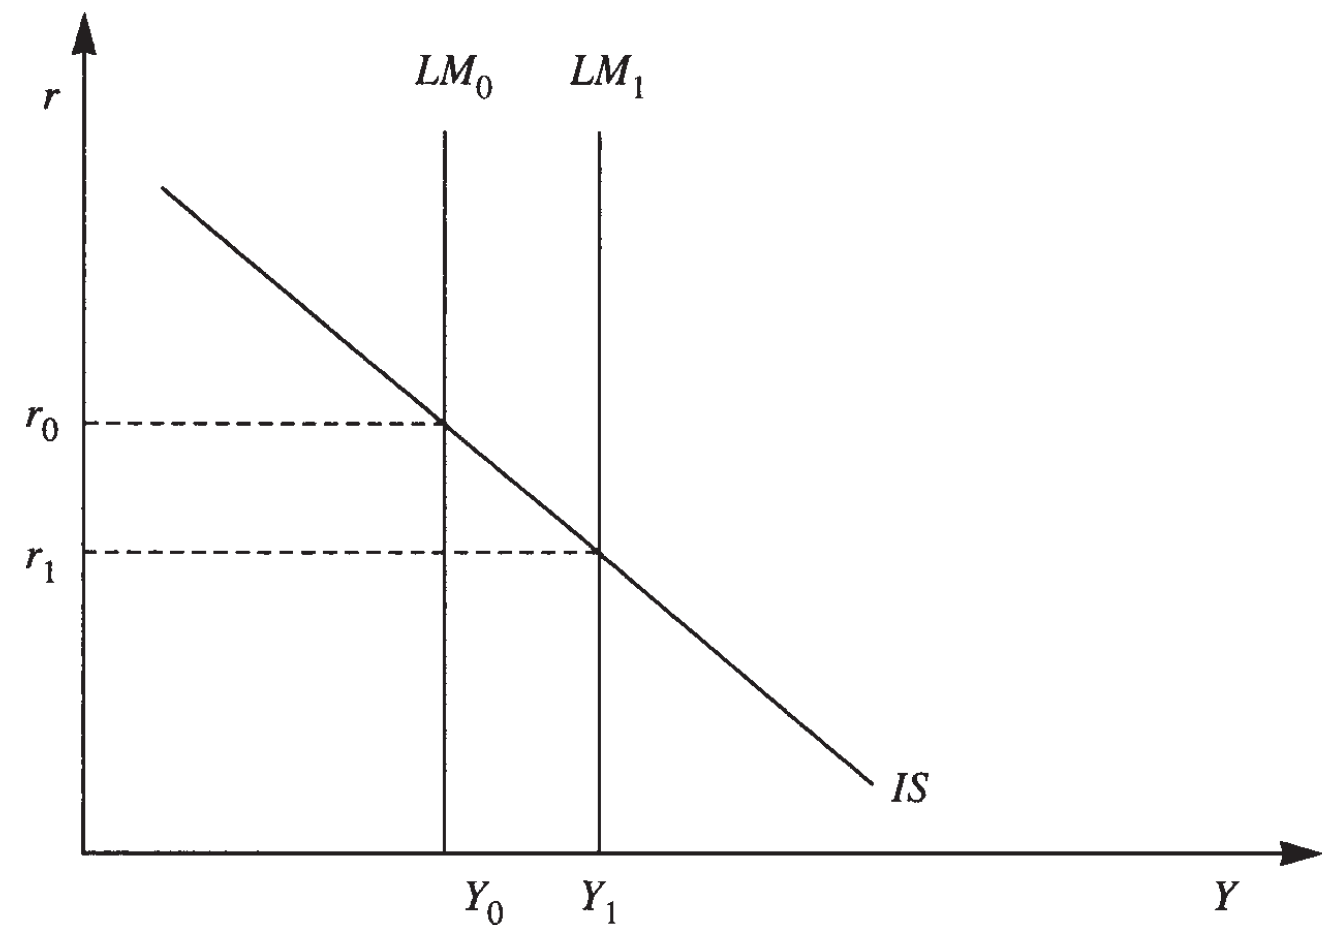
\includegraphics[width=0.6\textwidth]{./figures/aula10_fig6.PNG}
        \caption{Caso clássico. Fonte: Snowdon e Vane (2005).}
        \label{fig6}
    \end{figure}
\end{frame}

\begin{frame}{TQM e variações na renda nominal: evidência empírica}
    \begin{itemize}
        \item Fig. \ref{fig6}: caso clássico - demanda por moeda independente da taxa de juros
        \bigskip
        \item Inicialmente equilíbrio de subemprego $Y_0$ a uma taxa de juros $r_0$
        \bigskip
        \item $\uparrow$ oferta de moeda $\Rightarrow$ taxa de juros mais baixa ($r_1)$ e um nível de renda mais alto ($Y_1$)
        \bigskip
        \item À medida que a taxa de juros cai, os gastos com investimento são estimulados o que, por sua vez, via efeito multiplicador, afeta o consumo e a renda
        \bigskip
        \item No caso clássico, então, estudos empíricos evidenciariam relação estável entre gasto autônomo e nível de renda, mesmo que a direção de causalidade fosse da moeda para a renda
    \end{itemize}
\end{frame}

\begin{frame}{TQM e variações na renda nominal: evidência empírica}
    \begin{figure}
        \centering
        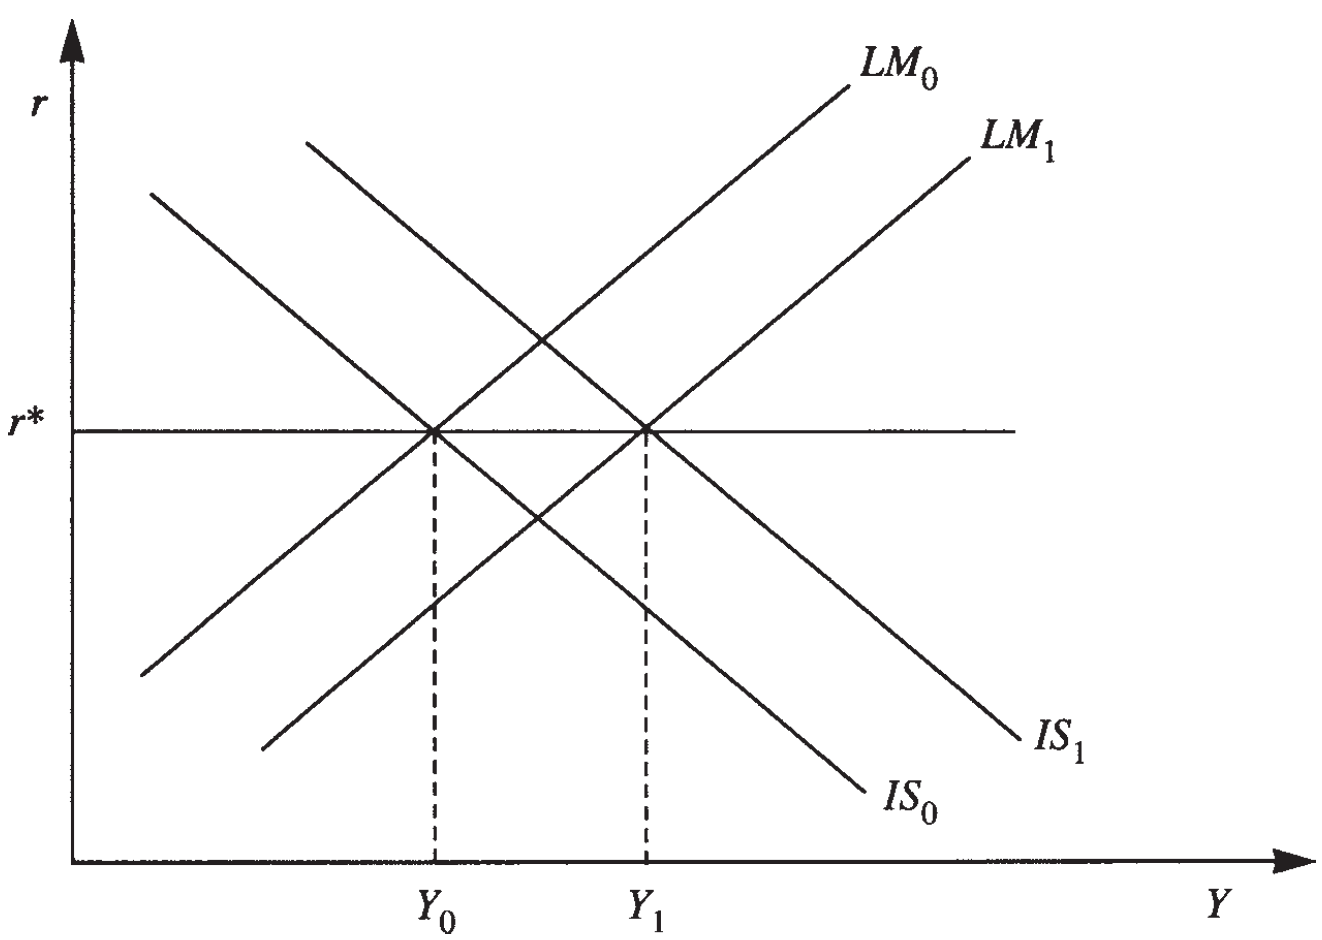
\includegraphics[width=0.6\textwidth]{./figures/aula10_fig7.PNG}
        \caption{Caso Keynesiano. Fonte: Snowdon e Vane (2005).}
        \label{fig7}
    \end{figure}
\end{frame}

\begin{frame}{TQM e variações na renda nominal: evidência empírica}
    \begin{itemize}
        \item Fig. \ref{fig7}: caso keynesiano
        \bigskip
        \item Inicialmente equilíbrio ao nível de renda $Y_0$ e taxa de juros $r^*$
        \bigskip
        \item Seguindo um impulso expansionário real, as autoridades estabilizariam a taxa de juros em $r^*$ expandindo a oferta de moeda
        \bigskip
        \item No caso Keynesiano, estudos econométricos evidenciariam uma relação estável entre oferta de moeda e nível de renda, mesmo que neste caso particular a direção de causalidade fosse da renda para a moeda
    \end{itemize}
\end{frame}

\begin{frame}{TQM e variações na renda nominal: evidência empírica}
    \begin{itemize}
        \item Concluindo, o que os testes Friedman-Meiselman demonstraram, aparentemente, foi que:
        \bigskip
        \begin{enumerate}
            \item A propensão marginal a consumir tem sido relativamente estável
            \bigskip
            \item Ao contrário da visão Keynesiana extrema, a economia não situa-se em uma situação de armadilha da liquidez porque, fosse este o caso, os testes não apresentariam uma boa performance para a equação que tem moeda como variável independente
        \end{enumerate}
    \end{itemize}
\end{frame}

\section{Principais proposições do monetarismo}
\begin{frame}{Principais proposições do monetarismo}
    \begin{enumerate}
        \item ``A teoria quantitativa é, em primeira instância, uma teoria de demanda por moeda'' (Friedman, 1956)
        \bigskip
        \item $\Delta$ no estoque de moeda fator predominante na explicação de $\Delta$ na renda nominal: ``Variações significativas nos preços ou na renda nominal são, quase sempre, o resultado de variações na oferta nominal de moeda'' (Friedman, 1968)
        \bigskip
        \begin{itemize}
            \item Proposição com duas implicações: (i) a maior parte dos ciclos tem origem monetária; (ii) inflação é sempre um fenômeno monetário
        \end{itemize}
        \bigskip
        \item Com função de demanda por moeda estável, a maior parte da instabilidade observada pode ser atribuída a flutuações na oferta de moeda induzida pelas autoridades monetárias. Portanto, o setor econômico privado é estável
    \end{enumerate}
\end{frame}

\begin{frame}{Principais proposições do monetarismo}
    \begin{enumerate}        
        \item[4.] Autoridades podem controlar oferta de moeda se desejaram, e caso o decidam, a trajetória da renda nominal será diferente de uma situação na qual a oferta de moeda é endógena
        \bigskip
        \item[5.] O lag entre variações no estoque de moeda e variações na renda nominal é longo e variável, de forma que tentativas de usar política monetária discricionária para estabilizar a economia poderia tornar-se desestabilizador
        \bigskip
        \item[6.] A oferta de moeda deveria ser guiada por política monetária com uma taxa de crescimento da moeda fixa alinhada com a taxa de crescimento do produto subjacente para assegurar estabilidade dos preços no longo prazo
    \end{enumerate}
\end{frame}

\section{Curva de Phillips aumentada pelas expectativas}
\subsection{Introdução}
\begin{frame}{Introdução}
    \begin{itemize}
        \item Aulas passadas vimos a incorporação da curva de Phillips por Keynesianos ortodoxos
        \bigskip
        \item Possibilitando a formulação de uma teoria de formação dos preços
        \bigskip
        \item Além disso, possibilitou a possibilidade de recomendações de políticas macroeco claras acerca de diferentes combinações possíveis de desemprego e inflação
        \bigskip
        \item 1960s foi, portanto, período importante para a teoria Keynesiana
        \bigskip
        \item O trade-off aparente entre inflação e desemprego, se estável, parecia atraente e, neste período, a política macro nos EUA visou explorá-lo para reduzir continuamente o desemprego
    \end{itemize}
\end{frame}

\begin{frame}{Introdução}
    \begin{figure}
        \centering
        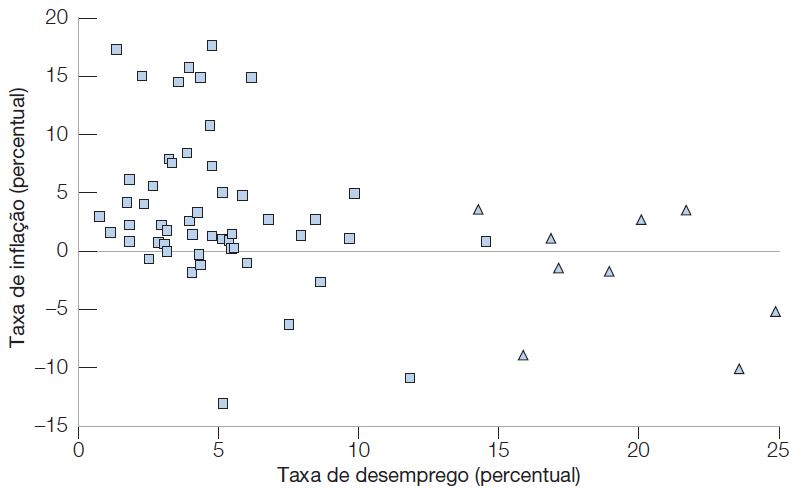
\includegraphics[width=0.7\textwidth]{./figures/aula10_fig8.JPG}
        \caption{Inflação $\times$ desemprego nos EUA, 1900-1960. Fonte: Blanchard (2017).}
        \label{fig75}
    \end{figure}
\end{frame}

\begin{frame}{Introdução}
    \begin{figure}
        \centering
        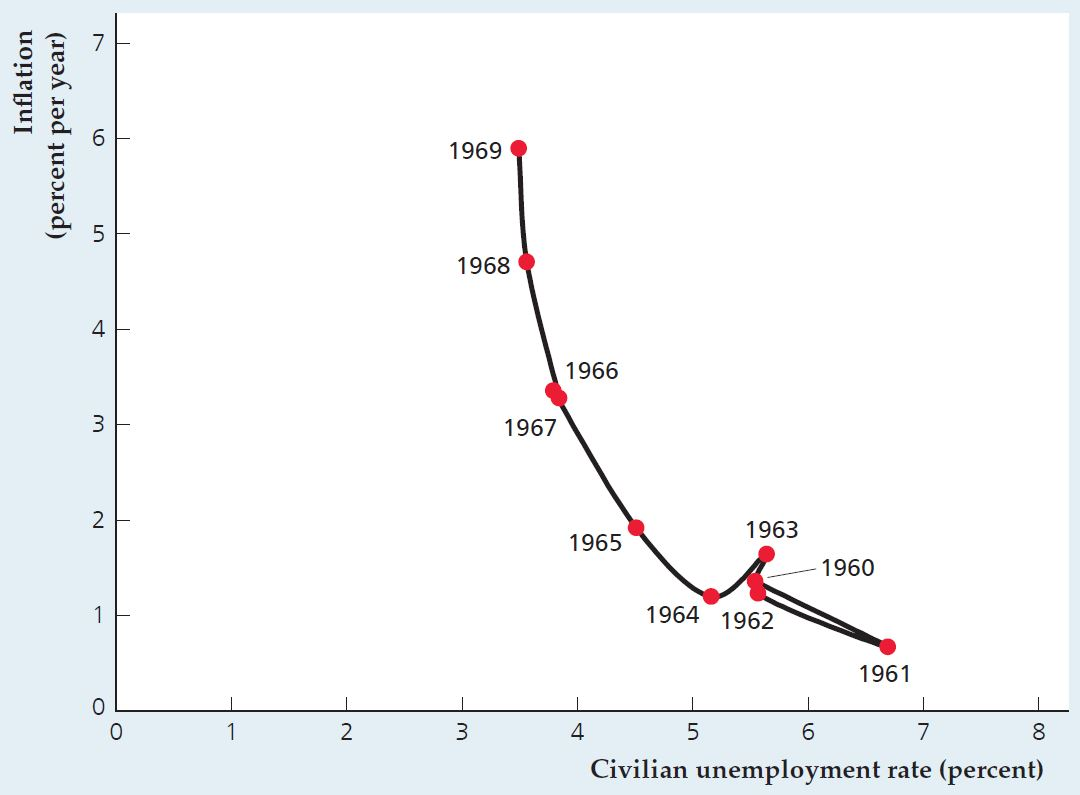
\includegraphics[width=0.6\textwidth]{./figures/aula10_fig9.JPG}
        \caption{Curva de Phillips e economia dos EUA durante a década de 1960. Fonte: Abel et al. (2017).}
        \label{fig8}
    \end{figure}
\end{frame}

\begin{frame}{Introdução}
    \begin{itemize}
        \item Fig. \ref{fig8}: como a relação entre desemprego e inflação se manteve durante a expansão econômica da década de 60
        \bigskip
        \item De 1961 a 1969, a taxa de desemprego baixou continuamente, de 6,8\% para 3,4\%
        \bigskip
        \item A taxa de inflação, por sua vez, subiu de aproximadamente 1\% para aproximadamente 6\%
        \bigskip
        \item De modo informal, a economia EUA deslocou-se para cima ao longo da curva de Phillips
        \bigskip
        \item Parecia que, se os formuladores de política econômica estivessem dispostos a aceitar uma inflação mais elevada, poderiam atingir um desemprego mais baixo
    \end{itemize}
\end{frame}

\begin{frame}{Introdução}
    \begin{itemize}
        \item Segundo estágio do monetarismo: análise mais precisa acerca da forma com que variações na taxa de uma expansão monetária são divididas entre magnitudes reais e nominais
        \bigskip
        \item Contribuições independentes de Friedman (1968) e Phelps (1967, 1968) à literatura da curva de Phillips (PC)
        \bigskip
        \item Uma relação estável entre inflação e desemprego foi questionada por Friedman e Phelps, que negaram a possibilidade de existência de um trade-off permanente (de longo-prazo) entre desemprego e inflação
        \bigskip
        \item Cabe ressaltar que a análise desenvolvida por Phelps teve origem em uma perspectiva não-monetarista
    \end{itemize}
\end{frame}

\begin{frame}{Introdução}
    \begin{itemize}
        \item Problema com especificação original da PC: taxa de variação dos salários nominais determinada de maneira independente da taxa de inflação
        \bigskip
        \item Isso implica que trabalhadores são irracionais e sofrem de ilusão monetária completa, dado que baseiam suas decisões de oferta de trabalho considerando apenas os salários nominais, de maneira independente do que acontece com os preços
        \bigskip
        \item A visão Keynesiana prevalente da curva de Phillips da década de 60 foi descreditada com ideias desenvolvidas ao final da década e acontecimentos dos 1970s
        \bigskip
        \item Os acontecimentos da década de 1970 deram razão a Friedman e Phelps em questionar a existência de um trade-off estável entre inflação e desemprego
    \end{itemize}
\end{frame}

\begin{frame}{Curva de Phillips aumentada por expectativas}
    \begin{figure}
        \centering
        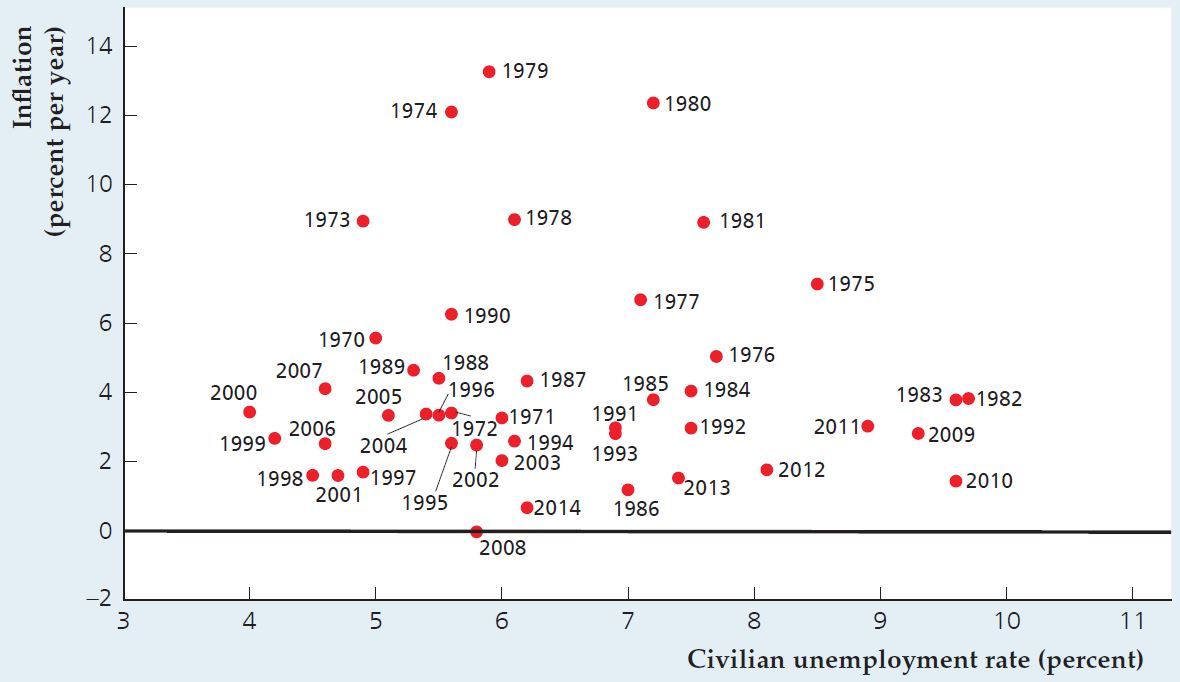
\includegraphics[width=0.8\textwidth]{./figures/aula10_fig10.JPG}
        \caption{Inflação e desemprego nos EUA, 1970-2014. Fonte: Abel et al. (2017).}
        \label{fig10}
    \end{figure}
\end{frame}

\begin{frame}{Curva de Phillips aumentada por expectativas}
    \begin{itemize}
        \item Friedman: PC original que relacionava taxa de variação dos salários nominais com desemprego mal-especificada
        \bigskip
        \item Salários nominais são determinados em negociações mas, empregadores e trabalhadores estão interessados nos salários reais
        \bigskip
        \item Dado que processos de barganha salarial são negociados para períodos de tempo discretos, o que influencia os salários reais antecipados é a \textcolor{purple}{taxa de inflação esperada} para o período do contrato de trabalho
    \end{itemize}    
\end{frame}

\begin{frame}{Curva de Phillips aumentada por expectativas}
    \begin{itemize}
        \item Friedman: PC deveria ser definida em termos de taxa de crescimento dos \textcolor{purple}{salários reais}
        \bigskip
        \item Portanto, PC original é aumentada com a taxa esperada (ou antecipada) de inflação como uma variável adicional determinante para a taxa de crescimento dos salários nominais
        \bigskip
        \item A \hlight{curva de Phillips aumentada por expectativas} pode ser expressa por:
        \begin{equation}
            \dot{W} = f(U) + \dot{P}^e
            \label{eq1}
        \end{equation}
        \bigskip
        \item A taxa de crescimento dos salários nominais é igual a um componente determinado pelo estado de excesso de demanda por trabalho (aproximado pelo nível de desemprego) somado à taxa de inflação esperada
    \end{itemize}    
\end{frame}

\begin{frame}{Curva de Phillips aumentada por expectativas}
    \begin{itemize}
        \item A incorporação da taxa de inflação esperada como variável adicional à proxy de excesso de demanda que determina a taxa de variação dos salários nominais implica que, ao invés de termos uma única PC temos, agora, uma família de curvas de Phillips, cada uma associada a um valor diferente de inflação esperada
        \bigskip
        \item Fig. \ref{fig11} ilustra duas PC possíveis
    \end{itemize}    
\end{frame}

\begin{frame}{Curva de Phillips aumentada por expectativas}
    \begin{figure}
        \centering
        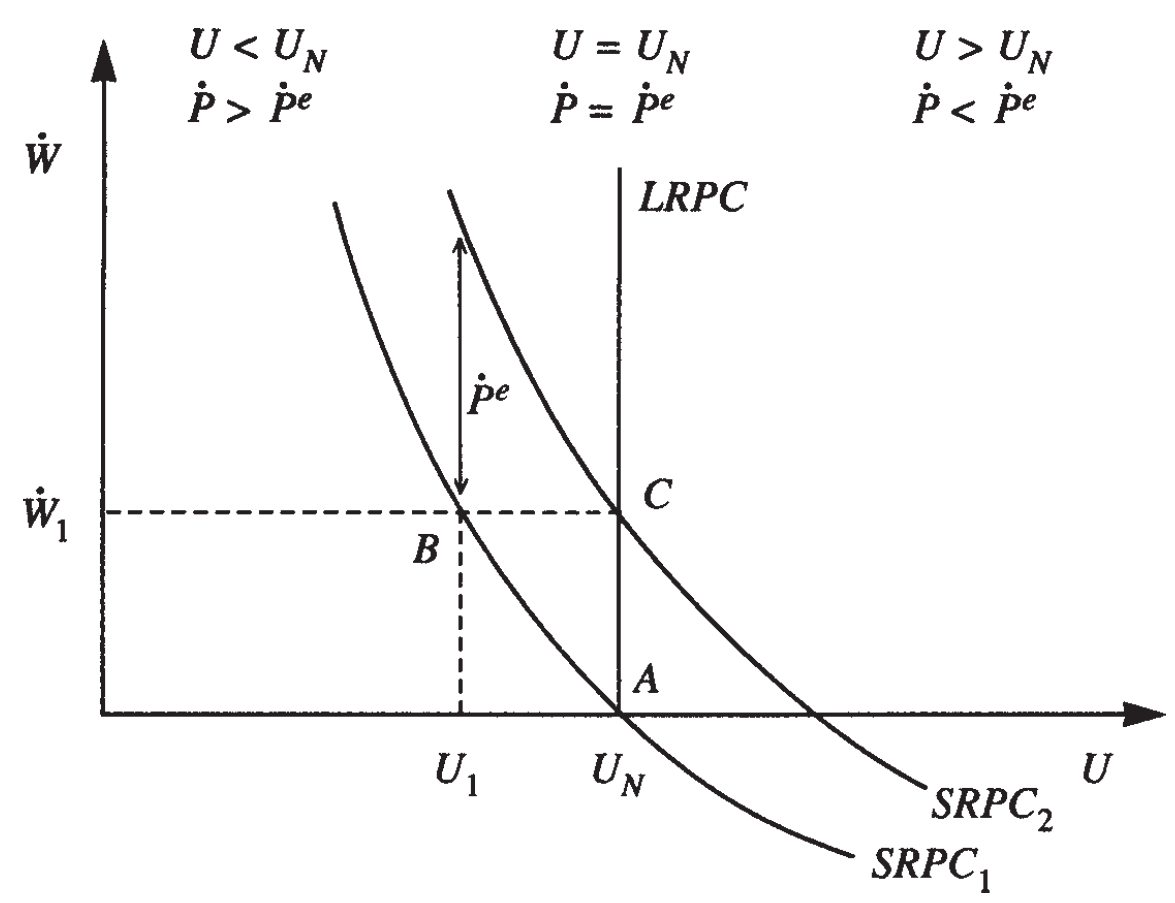
\includegraphics[width=0.6\textwidth]{./figures/aula10_fig11.PNG}
        \caption{Curva de Phillips aumentada por expectativas. Fonte: Snowdon e Vane (2005).}
        \label{fig11}
    \end{figure}
\end{frame}

\begin{frame}{Curva de Phillips aumentada por expectativas}
    \begin{itemize}
        \item Economia inicialmente em equilíbrio no ponto A ao longo da CP de curto prazo ($SRPC_1$) com desemprego em seu \textcolor{purple}{nível natural}, $U_N$, e taxa de crescimento de salários nominais nula
        \bigskip
        \item Hipótese: crescimento nulo de produtividade, de forma que $\dot{W} = \dot{P} = \dot{P}^e = 0\%$
        \bigskip
        \item Suponha que formuladores de política reduzam o desemprego de $U_N$ para $U_1$ via expansão de DA sob forma de aumento da base monetária
        \bigskip
        \item Excesso de demanda nos mercados de bens e serviços resultaria em pressão de alta sobre preços e salários nominais, com preços de mercadorias, tipicamente, se ajustando mais rápido que salários
    \end{itemize}    
\end{frame}

\begin{frame}{Curva de Phillips aumentada por expectativas}
    \begin{itemize}
        \item Tendo experienciado estabilidade de preços ($\dot{P}^e = 0$), trabalhadores entenderiam, erroneamente, o aumento de salário nominal como um aumento salarial real $\Rightarrow$ oferta de mão-de-obra aumenta
        \bigskip
        \item Ou seja, eles forem de ilusão monetária temporária
        \bigskip
        \item O salário real, no entanto, diminuiria e, à medida que as firmas demandam mais trabalho, a taxa de desemprego diminuiria, com salários nominais crescendo a uma taxa de $\dot{W}_1$ - ponto $B$
    \end{itemize}    
\end{frame}

\begin{frame}{Curva de Phillips aumentada por expectativas}
    \begin{itemize}
        \item À medida que trabalhadores comecem a revisar expectativas de inflação de forma compatível à inflação observada ($\dot{P} = \dot{W}_1$), perceberão que o salário real caiu e, portanto, pressionarão por um aumento de salários nominais
        \bigskip
        \item Essa pressão por aumento de salário nominal desloca a curva de Phillips de curto prazo de $SRPC_1$ para $SRPC_2$
        \bigskip
        \item Os salários nominais, então, crescem a uma taxa $\dot{W}_1$ somada à expectativa de taxa de inflação
        \bigskip
        \item As firmas, portanto, demitiriam trabalhadores à medida que o salário real aumenta e o desemprego aumentaria até que, no ponto $C$, os salários reais fossem restaurados ao seu nível original, com o desemprego retornando ao seu nível natural
    \end{itemize}    
\end{frame}

\begin{frame}{Curva de Phillips aumentada por expectativas}
    \begin{itemize}
        \item Portanto, quando a taxa efetiva de inflação é inteiramente antecipada ($\dot{P}_1=\dot{P}^e$) nas barganhas salariais ($\dot{W}_1 = \dot{P}^e$, i.e., não há ilusão monetária), \textcolor{purple}{não existirá um trade-off de longo prazo entre desemprego e inflação salarial}
        \bigskip
        \item Segue que se não há excesso de demanda (economia na \textcolor{purple}{taxa natural de desemprego}), então, a taxa de crescimento dos salários nominais será igual à expectativa de inflação
        \bigskip
        \item E apenas no caso particular em que a taxa de inflação esperada é igual a zero que a inflação salarial será nula - ponto $A$
        \bigskip
        \item Ao interpolarmos os pontos $A$ e  $C$, obtemos uma \textcolor{purple}{curva de Phillips de longo prazo} no nível de desemprego natural ($U_N$)
    \end{itemize}    
\end{frame}

\begin{frame}{Curva de Phillips aumentada por expectativas}
    \begin{itemize}
        \item Em $U_N$, a taxa de crescimento dos salários nominais é exatamente igual à taxa de crescimento dos preços, de forma que os salários reais são constantes
        \bigskip
        \item Consequentemente, não teremos distúrbios no mercado de trabalho
        \bigskip
        \item À taxa natural, o mercado de trabalho está em estado de equilíbrio e as taxas de inflação esperada e observada são iguais
        \bigskip
        \item Ou seja, a inflação é inteiramente antecipada
        \bigskip
        \item A análise de Friedman possibilitou reconciliar a proposição clássica de \textcolor{purple}{neutralidade da moeda no longo prazo, permitindo que a moeda tenha efeitos reais no curto prazo}
    \end{itemize}    
\end{frame}

\begin{frame}{Curva de Phillips aumentada por expectativas}
    \begin{itemize}
        \item Após crítica de Friedman à PC, estudos empíricos foram conduzidos acerca da PC aumentada por expectativas com o seguinte tipo de equação:
        \begin{equation}
            \dot{W} = f(U) + \beta \dot{P}^e
            \label{eq2}
        \end{equation}
        \bigskip
        \item Valores de $\beta$ estimados iguais à unidade implicam a inexistência de um trade-off de longo prazo
        \bigskip
        \item Valores estimados de $0<\beta<1$ implicam a existência de um trade-off de longo prazo, mas menos favorável que o existente no curto prazo
    \end{itemize}    
\end{frame}

\begin{frame}{Curva de Phillips aumentada por expectativas}
    \begin{figure}
        \centering
        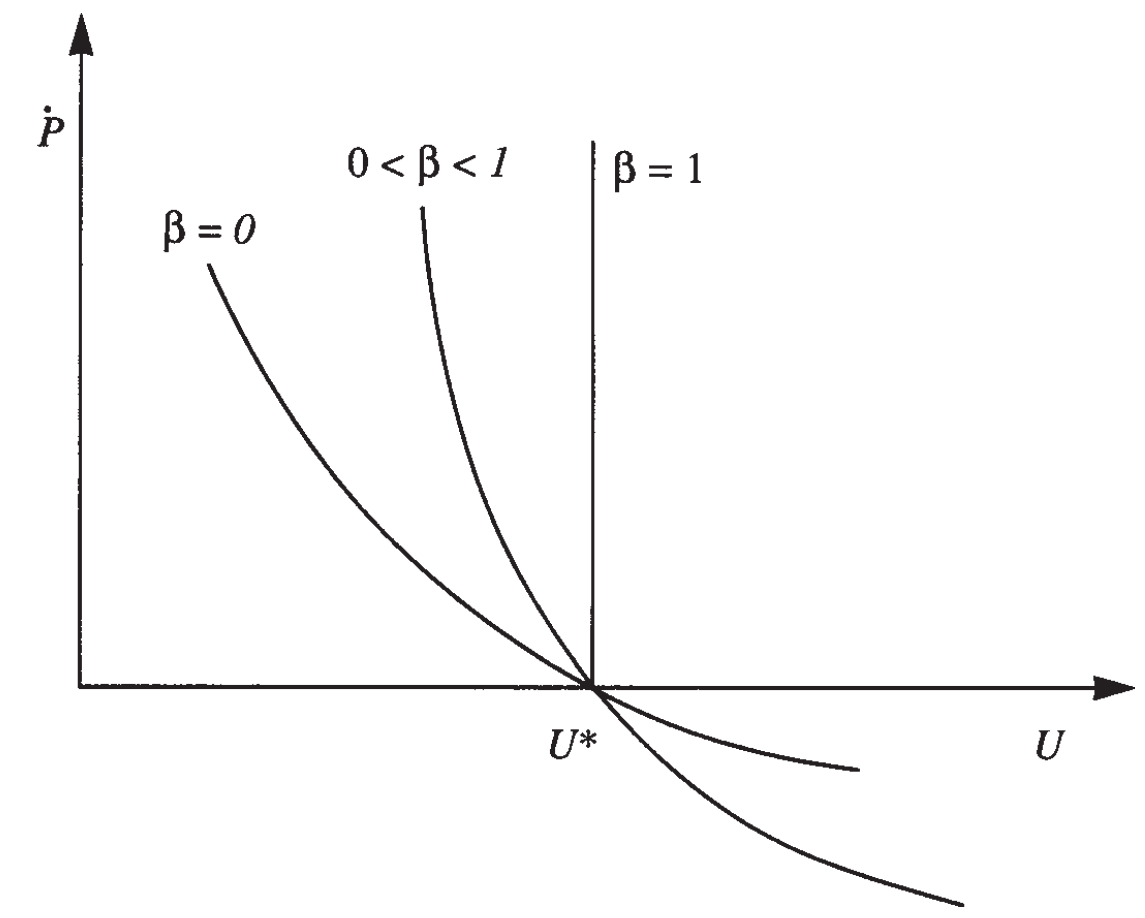
\includegraphics[width=0.55\textwidth]{./figures/aula10_fig12.PNG}
        \caption{Trade-off entre inflação e desemprego. Fonte: Snowdon e Vane (2005).}
        \label{fig12}
    \end{figure}
\end{frame}

\begin{frame}{Curva de Phillips aumentada por expectativas}
    \begin{itemize}
        \item As evidências dos estudos empíricos que objetivavam testar se o coeficiente estimado ($\beta$) no termo de expectativas de inflação é igual a um não são claras
        \bigskip
        \item Portanto, na década de 1970s, a possibilidade de existência de uma curva de Phillips de longo prazo vertical foi objeto de controvérsia entre Keynesianos e monetaristas
        \bigskip
        \item No entanto, ao final da década, a maioria dos economistas Keynesianos acabou aceitando que a PC de longo prazo é vertical
        \bigskip
        \item Há ainda, entretanto, controvérsias consideráveis no que diz respeito ao tempo necessário para a economia retornar ao longo prazo após ser submetida a algum distúrbio
    \end{itemize}    
\end{frame}

\begin{frame}{Curva de Phillips aumentada por expectativas}
    \begin{itemize}
        \item \textcolor{blue}{É possível uma curva de Phillips positivamente inclinada?}
        \bigskip
        \item (Memorial Nobel de 1977) PC positivamente inclinada pode ser compatível com uma PC de longo prazo vertical à taxa natural de desemprego:
        \bigskip
        \begin{enumerate}
            \item As taxas de inflação tendem a ficar mais voláteis quando inflação é muito elevada - aumenta incerteza e o desemprego pode emergir à medida que a eficiência de mercado é reduzida e o sistema de preços se torna menos eficiente como um mecanismo de coordenação/comunicação. Além disso, aumento da incerteza pode reduzir os investimentos e, com isso, aumentar desemprego
            \medskip
            \item Inflação elevada e mais volátil faz com que governos tomem medidas intervencionistas no processo de determinação de preços (controle de preços e salários) - reduz a eficiência do sistema de preços e resulta em desemprego
        \end{enumerate}
        \bigskip
        \item Uma relação positiva entre desemprego e inflação pode resultar de um aumento não-antecipado na taxa e volatilidade da inflação
    \end{itemize}    
\end{frame}

\subsection{Implicações de política econômica}
\begin{frame}{Implicações de política econômica}
    \begin{itemize}
        \item \textcolor{blue}{Escopo para ganhos de produto-emprego no curto prazo.} Hipótese monetarista de PC de longo prazo vertical implica que aumento na taxa de expansão monetária pode reduzir desemprego abaixo do natural apenas porque a inflação resultante não é antecipada pelos agentes
        \bigskip
        \item Se a inflação é completamente antecipada, ela será incorporada aos processos de barganhas salariais e, portanto, o desemprego retornará ao seu nível natural
        \bigskip
        \item A hipótese da análise monetarista é que a inflação esperada se ajusta à inflação observada apenas gradualmente, de acordo com o que conhecemos, hoje, por \textcolor{purple}{hipótese das expectativas adaptativas}
    \end{itemize}    
\end{frame}

\begin{frame}{Implicações de política econômica}
    \begin{itemize}
        \item A principal ideia por trás da hipótese de expectativas adaptativas é que os agentes econômicos adaptam suas expectativas acerca da inflação de acordo com as taxas de inflação passadas e, além disso, aprendem com seus erros
        \bigskip
        \item Assume-se que trabalhadores ajustem expectativas de inflação por uma fração do último erro cometido
        \bigskip
        \item Isto é, o diferencial entre a taxa de inflação observada e a taxa de inflação esperada:
        \begin{equation}
            \dot{P}_t^e - \dot{P}_{t-1}^e = \alpha (\dot{P}_t - \dot{P}_{t-1}^e),
            \label{eq3}
        \end{equation}
        onde $\alpha$ é uma fração constante
    \end{itemize}    
\end{frame}

\begin{frame}{Implicações de política econômica}
    \begin{itemize}
        \item Por método iterativo, a inflação esperada  pode ser obtida como média ponderada geométrica das inflações passadas observadas com um maior peso atribuído às experiências de inflação mais recentes:
        \begin{equation}
            \dot{P}_t^e = \alpha \dot{P}_t + \alpha(1-\alpha)\dot{P}_{t-1} + \dots + \alpha(1-\alpha)^n\dot{P}_{t-n}
            \label{eq4}
        \end{equation}
        \bigskip
        \item Neste modelo \textcolor{purple}{backward-looking}, as expectativas de inflação são baseadas apenas nas taxas de inflação observadas passadas
        \bigskip
        \item A existência de um hiato temporal entre um aumento na taxa de inflação e um aumento na taxa de inflação esperada possibilita uma redução temporária no desemprego abaixo do nível natural
    \end{itemize}    
\end{frame}

\begin{frame}{Implicações de política econômica}
    \begin{itemize}
        \item Se inflação é completamente antecipada, economia retorna para seu nível natural de taxa de desemprego, mas com uma taxa mais elevada de inflação de preços e de salários - igual à taxa de crescimento monetária
        \bigskip
        \item Como discutiremos mais tarde, sob \textcolor{purple}{hipótese de expectativas racionais} e se agentes econômicos tem mesmo conjunto de informação que as autoridades, então, a taxa de inflação esperada irá aumentar imediatamente em resposta a um aumento na taxa de expansão monetária
        \bigskip
        \item Neste caso em que não há hiato temporal entre aumentos na inflação observada e inflação esperada, as autoridades são impotentes para influenciar produto e emprego, mesmo no curto prazo
    \end{itemize}    
\end{frame}

\begin{frame}{Implicações de política econômica}
    \begin{itemize}
        \item \textcolor{blue}{A hipótese aceleracionista}. Qualquer tentativa de manter a taxa de desemprego \textcolor{purple}{permanentemente} abaixo da taxa natural resultará em uma aceleração da inflação e irá requerer que as autoridades continuamente aumentem a taxa de expansão monetária
        \bigskip
        \item Fig. \ref{fig11}: se desemprego fosse mantido permanentemente em $U_1$, a existência permanente de excesso de demanda no mercado de trabalho levaria a uma taxa observada de inflação maior que a esperada
        \bigskip
        \item À medida que a taxa observada de inflação aumenta, os agentes revisariam suas expectativas de inflação para cima (i.e., deslocando a SRPC para cima) o que, por sua vez, levaria a um aumento da taxa de inflação observada e assim por diante, levando a uma hiperinflação
    \end{itemize}    
\end{frame}

\begin{frame}{Implicações de política econômica}
    \begin{itemize}
        \item Em outras palavras, para manter um desemprego abaixo do nível natural, os salários reais deveriam ser mantidos abaixo do nível de equilíbrio
        \bigskip
        \item Para que isso aconteça, o nível de preços observado deve crescer a uma taxa mais acelerada que os salários nominais
        \bigskip
        \item Nessa situação, os trabalhadores empregados iriam revisar suas expectativas de inflação para cima e pressionariam por aumentos de salários nominais mais elevados o que, por sua vez, levaria a uma taxa de inflação observada mais alta
        \bigskip
        \item O resultado seria uma aceleração da inflação que demandaria aumentos contínuos na taxa de expansão monetária para acomodar o aumento contínuo da taxa de inflação
    \end{itemize}    
\end{frame}

\begin{frame}{Implicações de política econômica}
    \begin{itemize}
        \item Analogamente, se desemprego é mantido permanentemente acima do natural, ocorrerá uma deflação acelerada
        \bigskip
        \item A existência contínua de excesso de oferta no mercado de trabalho fará com que a taxa de inflação observada seja menor que a esperada
        \bigskip
        \item Os agentes, então, revisarão suas expectativas de inflação para baixo (deslocando para baixo a SRPC) o que, por sua vez, leva a uma taxa de inflação observada mais baixa e assim sucessivamente
    \end{itemize}    
\end{frame}

\begin{frame}{Implicações de política econômica}
    \begin{itemize}
        \item \textcolor{purple}{Segue que a taxa natural é o único nível de desemprego no qual uma taxa constante de inflação pode ser mantida}
        \bigskip
        \item Em outras palavras, no equilíbrio de longo prazo com economia no nível natural de desemprego, a taxa de expansão monetária irá determinar a taxa de inflação (assumindo uma taxa de crescimento constante do produto agregado e da velocidade da moeda) em linha com a abordagem da TQM
    \end{itemize}    
\end{frame}

\begin{frame}{Implicações de política econômica}
    \begin{itemize}
        \item \textcolor{blue}{Custos em termos de produto-emprego associados à redução de inflação}. Dada a proposição de que a inflação é, essencialmente, um fenômeno monetário propagado por um crescimento da moeda excessivo, monetaristas argumentam que a inflação só pode ser reduzida por uma desaceleração da taxa de crescimento da oferta de moeda
        \bigskip
        \item Isso, no entanto, resulta em um aumento no nível de desemprego
        \bigskip
        \item O dilema enfrentado pelos formuladores de política econômica é que o quão mais rápido desejarem reduzir a inflação via contração monetária, maiores serão os custos em termos de desemprego
    \end{itemize}    
\end{frame}

\begin{frame}{Implicações de política econômica}
    \begin{itemize}
        \item Alguns monetaristas advogam em favor de um processo de ajustamento gradual no qual a taxa de expansão monetária é reduzida ao nível desejado visando minimizar os custos de emprego-produto associados à redução da inflação
        \bigskip
        \item Fig. \ref{fig13} ilustra políticas alternativas de gradualismo e redução abrupta
    \end{itemize}    
\end{frame}

\begin{frame}{Implicações de política econômica}
    \begin{figure}
        \centering
        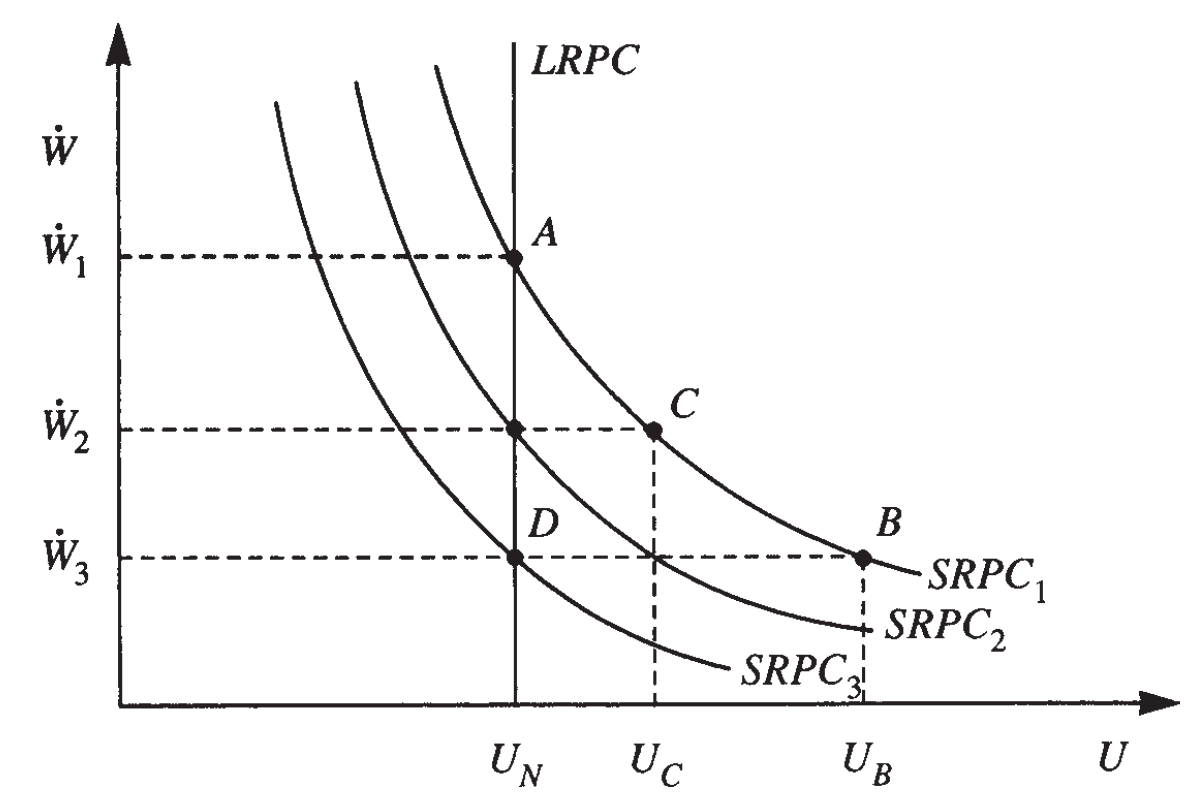
\includegraphics[width=0.65\textwidth]{./figures/aula10_fig13.PNG}
        \caption{Os custos de redução de inflação em termos de emprego-produto. Fonte: Snowdon e Vane (2005).}
        \label{fig13}
    \end{figure}
\end{frame}

\begin{frame}{Implicações de política econômica}
    \begin{itemize}
        \item Equilíbrio inicial determinado pelo ponto A de intersecção entre as curvas $SRPC_1$ e $LRPC$
        \bigskip
        \item Na posição inicial, economia em uma situação de equilíbrio de curto e longo prazos, no qual há uma taxa constante de inflação de preços e salarial que é completamente antecipada ($\dot{W}_1 = \dot{P} = \dot{P}^e$) e o desemprego está em seu nível natural
        \bigskip
        \item Suponha que a taxa de inflação é considerada pelas autoridades como alta e que desejem reduzir a taxa de inflação reduzindo a taxa de expansão monetária e mover-se para a posição D na LRPC
    \end{itemize}    
\end{frame}

\begin{frame}{Implicações de política econômica}
    \begin{enumerate}
        \item \textcolor{purple}{Redução abrupta}. É possível alcançar o ponto D via uma redução acentuada da taxa de expansão monetária. Desemprego aumentaria consideravelmente para $U_B$, de forma que a inflação de preços e salarial seja reduzida rapidamente para $\dot{W}_3$. O custo inicial dessa alternativa de política será um aumento relativamente alto no desemprego
        \bigskip
        \item \textcolor{purple}{Redução gradual}. O mesmo objetivo pode ser alcançado via redução inicial menor na taxa de expansão monetária e um aumento do desemprego para $U_C$ - inflação será reduzida, inicialmente, para $\dot{W}_2$ ao longo da curva $SRPC_1$. Uma redução subsequente na taxa de expansão monetária pode reduzir ainda mais a taxa de inflação até o ponto em que a meta de inflação $\dot{W}_3$ seja alcançada
    \end{enumerate}    
\end{frame}

\begin{frame}{Implicações de política econômica}
    \begin{itemize}
        \item No caso de uma redução gradual, o intervalo temporal para que a transição de uma taxa de inflação de $\dot{W}_1$ seja reduzida para $\dot{W}_3$ é muito maior que no caso de uma redução abrupta
        \bigskip
        \item Tais medidas de política, então, implicam que os agentes econômicos terão de conviver por um longo período de tempo com taxas de inflação elevadas
        \bigskip
        \item Por esse motivo, muitos economistas defendem o uso de políticas suplementares que acompanhem esse processo de ajuste gradual para uma taxa de inflação mais baixa
    \end{itemize}    
\end{frame}

\begin{frame}{Implicações de política econômica}
    \begin{itemize}
        \item Antes de considerarmos o escopo de utilização de políticas complementares, é importante ressaltarmos a importância que a credibilidade tem para qualquer estratégia de política antiinflacionária - assunto que discutiremos com maior profundidade ao analisarmos a escola novo-clássica
        \bigskip
        \item Se os agentes econômicos acreditam que as autoridades estão comprometidas com políticas monetárias contracionistas para reduzir a inflação, eles revisarão suas expectativas inflacionárias para baixo de maneira mais rápida e, portanto, reduzirão os custos em termos de produto-emprego associados ao processo de ajuste
    \end{itemize}    
\end{frame}

\begin{frame}{Implicações de política econômica}
    \begin{itemize}
        \item Políticas suplementares ao processo de ajuste gradual:
        \bigskip
        \begin{enumerate}
            \item \textcolor{purple}{Indexação}. Pode reduzir não apenas os custos de inflação não-antecipada que ocorrem por uma redistribuição arbitrária da renda e riqueza mas, também, os custos de emprego-produto associados à redução na taxa de expansão monetária
            \bigskip
            \begin{itemize}
                \item Com indexação, aumentos de salário nominal iriam declinar automaticamente com qualquer aumento inflacionário e, assim, removendo o risco de que trabalhadores se comprometeriam, sob os contratos existentes, a aumentos excessivos de salários nominais quando a inflação é reduzida
                \bigskip
                \item Em outras palavras, com indexação, aumentos salariais ocorreriam em uma velocidade menor e o desemprego aumentaria, então, em uma magnitude menor
            \end{itemize}
        \end{enumerate}
    \end{itemize}    
\end{frame}

\begin{frame}{Implicações de política econômica}
            \begin{enumerate}            
            \item[2.] \textcolor{purple}{Políticas de preços e de renda.} Alguns economistas (e.g., Tobin, Trevithick e Stevenson) argumentam que políticas de preços e de renda poderiam ter um papel importante, como políticas temporárias e suplementares à contração monetária, para ajudar no processo de transição para uma taxa de inflação mais baixa ao reduzir as expectativas inflacionárias.
            \bigskip
            \begin{itemize}
                \item Em termos da Fig. \ref{fig13}, as PCs de curto prazo seriam deslocadas para baixo de forma mais rápida
                \bigskip
                \item Isso permitiria que o ajuste a uma taxa de inflação mais baixa pudesse ser atingido de maneira mais rápida e com custos menores em termos de magnitude e duração do desemprego que acompanha a contração monetária
                \bigskip
                \item No entanto, um problema com essas medidas suplementares é que, mesmo que a política tenha sucesso em reduzir as expectativas inflacionárias, uma vez retirada, as expectativas podem ser revisadas para cima - SRPC desloca para cima compensando o benefício inicial da política adotada
            \end{itemize}
        \end{enumerate}    
\end{frame}

\begin{frame}{Implicações de política econômica}
    \begin{itemize}
        \item Em resumo, os custos em termos de emprego-produto associados a uma contração monetária dependem de três fatores:
        \bigskip
        \begin{enumerate}
            \item Se as autoridades adotam uma redução na taxa de expansão monetária de forma gradual ou abrupta
            \bigskip
            \item A extensão das adaptações institucionais, e.g., se os contratos salariais são indexados ou não
            \bigskip
            \item A velocidade com que os agentes econômicos reduzem suas expectativas inflacionárias
        \end{enumerate}
    \end{itemize}    
\end{frame}

\begin{frame}{Implicações de política econômica}
    \begin{itemize}
        \item \textcolor{blue}{Papel e condução da política monetária}. A crença em uma LRPC vertical e de que políticas de DA podem ter um efeito sobre o nível de produto e de emprego apenas no curto prazo tem implicações importantes para o papel e condução da política monetária
        \bigskip
        \item A prescrição de política econômica de Friedman para uma taxa de crescimento da moeda constante (combinada com uma taxa de câmbio flexível), em linha com a tendência de taxa de crescimento de longo prazo da economia, é baseada em vários argumentos:
        \bigskip
        \begin{enumerate}
            \item Se as autoridades expandem a oferta de moeda a uma taxa estacionária ao longo do tempo, a economia tende a se equilibrar na taxa natural de desemprego com uma taxa de inflação estacionária, i.e., ao longo da curva de Phillips de longo prazo vertical
        \end{enumerate}
    \end{itemize}    
\end{frame}

\begin{frame}{Implicações de política econômica}
            \begin{enumerate}            
            \item[2.] A adoção de uma regra monetária removeria a principal fonte de instabilidade na economia, ou seja, as economias capitalistas avançadas são inerentemente estáveis ao redor da taxa natural de desemprego, a não ser que sejam atingidas por crescimentos monetários erráticos
            \bigskip
            \item[3.] Políticas discricionárias poderiam ser desestabilizantes, dado o hiato longo e variável associado à política monetária
            \bigskip
            \item[4.] Como a taxa natural é uma variável não-observável (que pode variar ao longo do tempo), o governo não deveria perseguir uma meta de taxa de desemprego pois isso poderia levar a um processo aceleracionista de inflação
        \end{enumerate}
    
\end{frame}

\begin{frame}{Implicações de política econômica}
    \begin{itemize}
        \item \textcolor{blue}{Taxa natural de desemprego e políticas do lado da oferta}. A taxa natural de desemprego é associada ao equilíbrio no mercado de trabalho e, portanto, à estrutura das taxas de salários reais
        \bigskip
        \item Friedman define a taxa natural como:
        \NB{
            O n\'{i}vel que seria determinado pelo sistema de equa\c{c}\~{o}es de equil\'{i}brio geral Walrasiano, desde que nele estejam embutidos as caracter\'{i}sticas estruturais dos mercados de trabalho e de bens, incluindo imperfei\c{c}\~{o}es de mercado, varia\c{c}\~{o}es estoc\'{a}sticas de demanda e oferta, o custo de coleta de informa\c{c}\~{o}es de vagas de emprego dispon\'{i}veis, os custos de mobilidade, e assim por diante
        
        \begin{flushright}
            (Friedman, 1968)
        \end{flushright}}
    \end{itemize}    
\end{frame}

\begin{frame}{Implicações de política econômica}
    \begin{itemize}
        \item Em outras palavras, a taxa natural de desemprego não é uma constante numérica, mas se apoia em fatores reais em oposição aos monetários: a eficácia do mercado de trabalho; o nível de competição ou monopólio; os obstáculos ou incentivos ao trabalho em várias ocupações; etc
        \bigskip
        \item Portanto, se governos desejam reduzir a taxa natural de desemprego de forma a atingir níveis de produto e de emprego mais elevados, deveriam focar em políticas de oferta que sejam formuladas para melhorar a estrutura e funcionamento do mercado de trabalho, ao invés de políticas de demanda
    \end{itemize}    
\end{frame}

\begin{frame}{Implicações de política econômica}
    \begin{itemize}
        \item Exemplos de políticas de oferta (controversas) que foram adotadas ao longo da década de 1980s incluem medidas que visavam aumentar:
        \bigskip
        \begin{enumerate}
            \item Os incentivos ao trabalho, e.g., reduções nas alíquotas de imposto de renda marginal e reduções nos benefícios de seguridade social e seguro-desemprego
            \bigskip
            \item Práticas de flexibilização de salários e relações trabalhistas, e.g., reduzindo a força dos sindicatos
            \bigskip
            \item Mobilidade ocupacional e geográfica do trabalho, e.g., maior oferta governamental de esquemas de treinamento
            \bigskip
            \item Eficiência dos mercados de bens e serviços, e.g., através de privatizações
        \end{enumerate}
    \end{itemize}    
\end{frame}

\begin{frame}{Implicações de política econômica}
    \begin{itemize}
        \item O conceito de taxa natural de desemprego é controverso
        \bigskip
        \item Além disso, tem sido definido de várias maneiras distintas
        \bigskip
        \item Como identificado por Rogerson (1997), a taxa natural tem sido definida como de ``longo prazo = friccional = média = equilíbrio = normal = pleno emprego = estado estacionário = mais baixa sustentável = eficiente = tendência de Hodrick-Prescott = natural''
        \bigskip
        \item Esses problemas de definição fizeram com que economistas preferissem usar o conceito de NAIRU - \textcolor{purple}{taxa de desemprego não-aceleradora de inflação}
        \bigskip
        \item Enquanto grande parte dos economistas admitam que é ``difícil pensar em políticas macroeconômicas sem o conceito de NAIRU'' (Stiglitz, 1997), muitos permanecem convencidos de que o conceito de taxa natural não é útil, e.g., Galbraith, Arestis, Sawyer e Akerlof
    \end{itemize}    
\end{frame}

\section{Bibliografia}
\begin{frame}{\emoji{books} Bibliografia}
    \begin{itemize}   
        \item ABEL, A.; BERNANKE, B.; CROUSHORE, D. Macroeconomics. 9.ed. Pearson Prentice Hall, 2017\medskip        
        \item ANDO, A.; MODIGLIANI, F. The Relative Stability of Monetary Velocity and the Investment Multiplier, American Economic Review, 1956 \medskip
        \item BLANCHARD, O. Macroeconomia. 7.ed. São Paulo: Pearson Education do Brasil, 2017\medskip                     
        \item CULBERTSON, J.M. FRIEDMAN on the Lag in Effect of Monetary Policy, Journal of Political Economy \medskip
        \item CULBERTSON, J.M. The Lag in Effect on Monetary Policy: Reply, Journal of Political Economy, 1961 \medskip
        \item DE PRANO, M.; MAYER, T. Tests of the Relative Importance of Autonomous Expenditure and Money, American Economic Review, 1965 \medskip
        \item FRIEDMAN, M. The Quantity Theory of Money, A Restatement, in M. FRIEDMAN (ed.), Studies in the Quantity Theory of Money, Chicago: University of Chicago Press, 1956 \medskip
        \item FRIEDMAN, M. The Supply of Money and Changes in Prices and Output, reprinted in The Optimum Quantity of Money and Other Essays, Chicago: Aldine, 1958 \medskip        
    \end{itemize}
\end{frame}

\begin{frame}{\emoji{books} Bibliografia}
    \begin{itemize}                        
        \item FRIEDMAN, M. The Demand for Money – Some Theoretical and Empirical Results, Journal of Political Economy, 1959 \medskip
        \item FRIEDMAN, M. The Role of Monetary Policy, American Economic Review, 1968 \medskip
        \item FRIEDMAN, M. Money: Quantity Theory, in D. Sills (ed.), The International Encyclopedia of the Social Sciences, New York: Macmillan Free Press, 1968 \medskip
        \item FRIEDMAN, M. Nobel Lecture: Inflation and Unemployment, Journal of Political Economy, 1977 \medskip
        \item FRIEDMAN, M.; MEISELMAN, D. The Relative Stability of Monetary Velocity and the Investment Multiplier in the United States, 1897–1958, in Commission on Money and Credit: Stabilization Policies, Englewood Cliffs, NJ: Prentice-Hall, 1963 \medskip
        \item FRIEDMAN, M.; SCHWARTZ, A.J. A Monetary History of the United States, 1867–1960, Princeton: Princeton University Press, 1963 \medskip
        \item KAREKEN, J.; SOLOW, R.N. Monetary Policy: Lags versus Simultaneity, in Commission on Money and Credit: Stabilization Policies, Englewood Cliffs, NJ: Prentice-Hall, 1963 \medskip        
    \end{itemize}
\end{frame}

\begin{frame}{\emoji{books} Bibliografia}
    \begin{itemize}                        
        \item MCDONALD, J.F. Rethinking Macroeconomics: a history of economic thought perspective. 2.ed. Routledge, 2022\medskip
        \item PHELPS, E.S. Phillips Curves, Expectations of Inflation and Optimal Unemployment Over Time, Economica, 1967 \medskip
        \item PHELPS, E.S. Money Wage Dynamics and Labour Market Equilibrium, Journal of Political Economy, 1968 \medskip
        \item ROGERSON, R. Theory Ahead of Language in the Economics of Unemployment, Journal of Economic Perspectives, 1997 \medskip
        \item SNOWDON, B.; VANE, H.R. \emph{Modern Macroeconomics: its Origins, Development and Current State}. Northampton, MA: Edward Elgar, 2005\medskip        
        \item STIGLITZ, J.E. Reflections on the Natural Rate Hypothesis, Journal of Economic Perspectives, 1997 \medskip
        \item TOBIN, J. Money and Income: Post Hoc Ergo Propter Hoc, Quarterly Journal of Economics, 1970 \medskip        
    \end{itemize}
\end{frame}

\end{document}